\documentclass{article}


\usepackage[margin=1in, left=1.5in, includefoot]{geometry} 
\usepackage{amsmath}
\usepackage{gensymb}
\usepackage{parskip}
\usepackage[none]{hyphenat}

%graphic stuff

\usepackage{graphicx} % allows images

\usepackage{float} %helps with posisioning


%header and footer stuff

\usepackage{fancyhdr}

\pagestyle{fancy}

\fancyhead{}

\fancyfoot{}

\fancyhead[L]{Robotic Artist:Walter / 0.1 (WIP)}

\fancyfoot[L]{Aberystwyth University / Computer Science}

\fancyfoot[R]{page: \thepage}

\renewcommand{\headrulewidth}{0pt}

\renewcommand{\footrulewidth}{0pt}


%begins document

 \begin{document}



    % begin title screen

    \begin{titlepage}

        \begin{center}

        \line(1,0){340}\\ 


        \large{\bfseries Robotic Artist:Walter} \\

        \large {\bfseries G400 Computer Science, CS39440 }\\
        
        \large {\bfseries Final Report}\\


         \line(1,0){250}\\

         \textsf {Author: Matthew Howard \\
          Candidate Number: 150035512\\
          User ID: Mah60 \\
          Supervisor Name: Helen Miles \\
          Supervisor ID: Hem23\\
          Last Modified: 29/04/2018 \\
          Version: 0.1\\
          Status: Work In Progress(WIP)} \\

        \end{center}        

    \end{titlepage}
  
    \clearpage

 	\tableofcontents
 	
 	\clearpage
    \section{Introduction}
    
This document is the final report for the project 'Robotic Artist : Walter'. The purpose of this document is to talk about how the project was ran and excuted, describing the problems that was encounted during implementation, design and testing stages of the project. The final outcome at the end of the document will be evaluated and discussed how the project could of been improved overall. Then plans of future developments will also be discussed and how the project has been designed to make future development plans easier to be done.\\ \newline
 
    \subsection{Project Description}
    
The project that has been undertaken is to develop a 'Robotic Artist' from the Roland 990 Pen Plotter. This is a device that has been collecting dust within the department building for a few years now and the project has been undertaken to bring the device back to life.\\ \newline
Then the 'Paul the Robot' project\cite{Paul_the_robot} was what inspired the design and development of this project. The idea is to be able to develop a robot that can take a captured image of someones face and create an artistic drawing from that picture. Figure \ref{fig:paul_the_robot} demonstrates what 'Paul' was capable of drawing. This then lead to the idea of the project that has been developed and completed over the past few months. \\ \newline

\begin{figure}[h]
    \centering
    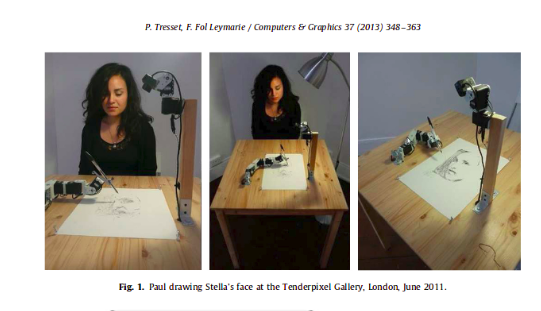
\includegraphics[width=0.65\textwidth]{Paul_the_robot.png}
    \caption{This figure is taken from the 'Paul the robot' article\cite{Paul_the_robot}. The article talks about a project that developed a abstract robotic artist, meaning the robot could draw out someone's face without knowing any of their facial features.}
    \label{fig:paul_the_robot}
\end{figure}

The main requirements of this project was to be able convert the Roland 990 Pen plotter to be able to plot out artistic drawings of peoples faces. So the next stage of the project was to understand what was required to be able to develop such an artist and what form of method would be undertaken to do this.\\ \newline

	\clearpage
	\section{Background and Anaylisis}
The background of the project came from the 'Paul the robot' project\cite{Paul_the_robot} as discussed in the introduction of this document. From this article the development of the Robotic artist came to be. The idea for this was to make a robotic artists using the Roland 990 Pen Plotter.\\ \newline
The idea of the project is to use image processing to generate an artistic style algorithm that is able to be plotted out on the Roland 990 plotter. This will involve generating an ideal method of looking into the image and then anaylising them in a way that enables the image to be transformed. One way of doing this would to look into the library 'OpenCv' that has been designed to do image processing and capture techniques. This library and the components that were given to the projects development, help to mold the start of the development of the project.\\ \newline
This is because 'OpenCv'\cite{OpenCv} is used mainly in two different languages Python or C. There has recently been a reach out to Java, however, the library for OpenCv is currently not well documented as that development is very recent. The development of OpenCv was to make it so the image processing techniques such as; looking at pixels, gaussian blur and canny edge dectection. These techniques are very useful when trying to process individual images as you can find patterns and features in a image that could be used to develop an artistic algorithm. Another, use of OpenCv is that it simplifies the technical work towards creating a working camera feed and image capturing techniques. This therefore makes OpenCv a valuable resource to be used within the project and was put into key account when anaylising how the project will be developed. \\ \newline
   
   \begin{figure}[h]
    \centering
    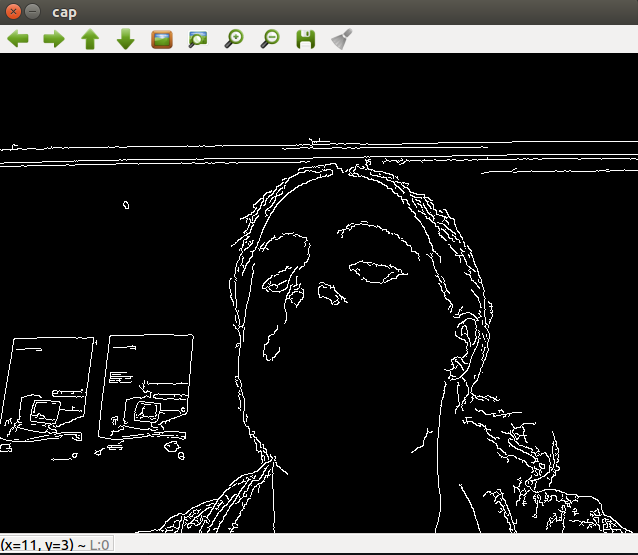
\includegraphics[width=0.4\textwidth]{canny_edge_example.png}
    \caption{Demonstrates OpenCv\cite{OpenCv} being used to apply the canny edge detection algorithm against a image. The image was taken as well, from using Open Cv to capture a frame the video camera.}
    \label{fig:canny_edge_detection}
	\end{figure}

The next part that helped to make a descision on how the projects final outcome came about was the components that were given to the project, to help achieve the final goal. These were the use of a Raspberri Pi 3, a web camera and a monitor with a mouse and keyboard. These key components are important as they defined the structure of the robot was given and how the components communicated with each other. \\ \newline
\clearpage
The initial ideas towards the components are explained are; \\ \newline
\begin{itemize}
  \item The Raspberri Pi would act as a controller that would help make the overall decisions on what would be done and then communcate to the individual devices give a output that was generated from the input from the monitor.
  \item The web camera would either be a standard camera or pi camera as it is designed to work with the Raspberri pi. This camera will capture multiple frames a second to display on the monitor in a form of graphical unit interface(GUI) and will capture an image when commanded to.
  \item The monitor will be there to display any video capture that is required for the robot and control any input from the user. The monitor will also display a gui, which will control the events that are occouring within the robot.
\end{itemize}

This set up that was given to the project for development based the structure of the code and gave the project a straight forward directions to take it. The overall robot design was not going to be like 'Paul the robot'\cite{Paul_the_robot}, however, would take the genral concepts and work around what was equipment was given to the project. For example Paul had a robotic arm that was designed to copy drawing styles of a human hand but this cannot be done with a pen plotter. Other concepts that could of been taken into account at the time of the design is whether to use a Raspberri Pi or a Arduino that would of been programmed in a form of C or another form of computer hardware.\\ \newline 
So therefore, the initial design for the project was to create a image processor that would use artistic style algorithms to generate an image that could then be translated into commands to be plotted out on the pen plotter. This lead to the development of the following features/requirements that can be seen in the requirement specifications\cite{Requirement_specifications}. \\ \newline  

 \begin{figure}[h]
    \centering
    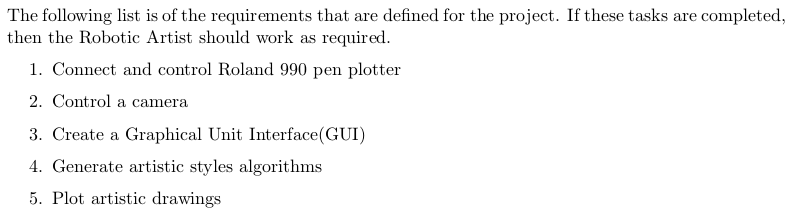
\includegraphics[width=0.7\textwidth]{requirements.png}
    \caption{This is a snippet of text from the Requirement Specifications\cite{Requirement_specifications} tha demonstrates the key requirements for this project. The requirements are exapanded upon within the document itself.}
    \label{fig:requirements}
	\end{figure}

These requirements in Figure \ref{fig:requirements} are the key features that will need to be implimented into the final project to achieve the optimal outcome. The overall idea was to make a graphical unit interface(GUI) with four key stages that would control the events that were occouring within the robot. These are video capture, picture accepance, style selectiong and style confirmation pages. This would allow the user to take and confirm the image is appropriate for use. Then they would be able to select from a range of artistic style, to tranform there image to. This would then let the user see the final output before plotting the style.\\ \newline
The next stage of the project was to research into the different methods of completing the key requirement and to then decide on which method would give the most optimal output.\\ \newline
\clearpage
	\subsection{Research}
	Notes =>  talk about how design choices was made as the individual requirements was being looked at. How modifications were made thoughout the project.
	what language to use
 	Which gui platform to use
 	How to communicate with the plotter - using serial instead of switch - look at 		
 						manual
 			- Once the connection was made, looking into individual commands and how 	
 			the plotter worked as a whole.
  	
 	
	\clearpage
	\section{Process/Methodology}
	
	\clearpage
	\section{Technical Work}
	
	\clearpage
	\section{Future Development}
	
	\clearpage
	\section{Critical Evaluation and Insight}
	
	\clearpage
    \section{Versions}


\begin{center}

\begin{tabular}{| l | p{8cm} | p{3cm}|}

\hline

\textbf{Version} & \textbf{Description} & \textbf{Date Modified} \\\hline

0.1 & Set up the basic Documentation layout. This includes creating the content and the individual chapters & 28/04/18 \\ \hline


\end{tabular}

    \begin{thebibliography}{9}

    \bibitem{Test_Plan}

    Matthew Howard (mah60);Test Plan; 25/04/2018 \\ 
    
    This document talks about the testing specifications that are used throughout this document.\\ 
    
    \bibitem{Requirement_specifications}

    Matthew Howard (mah60);Requirement Specifications; 25/04/2018 \\ 
    
    This document talks about the requirements that have been given to robotic artist project. The document can be found in the Appendices for this project.\\ 
    
    \bibitem{Paul_the_robot}

    Patrick Tresset, Frederic Fol Leymarie, Goldsmiths College ; "Portrait drawing by Paul the robot"; 28/04/2018 \\ 

    \textit{http://doc.gold.ac.uk/~ma701pt/patricktresset/wp-content/uploads/2015/03/computerandgraphicstresset.pdf}

This is the main article that I will be using throughout the project, as it was where the idea from the project came from and talks about different methods and styles when it comes to developing robotic artists. Such as, splitting the image into different sections and developing different consistences to pick out the lines and the shadows. Also it has references to other projects that are just like this one. 
 
 	\bibitem{OpenCv}

	OpenCv Documentation; OpenCv tutorials; 29/04/18 \\ 	
 	
 	\textit{https://docs.opencv.org/3.0-beta/doc/py\_tutorials/py\_tutorials.html}
 	
This resource talks about individual components that can be done with open cv to calculate image processing techniques. This site is a tutorial on how to use multiple of those techniques. \\
    
    \bibitem{qt_designer}

    QT Documentation;QT Designer Manual; 26/04/2018 \\ 
    
    \textit{http://doc.qt.io/qt-5/qtdesigner-manual.html}
    
    This site is a manual on how to use the Qt Designer software and demonstrates the software that was used to develop the GUI in this project.\\ 
    
    \bibitem{pyqt}

    Python Wiki;Pyqt4 library; 26/04/2018 \\ 
    
    \textit{https://wiki.python.org/moin/PyQt4}
    
    This site talks about the pyqt library that I used to develop the GUI. As well, provides learning materials to understand the library.\\ 

    \end{thebibliography}

\end{center}

 \end{document}